\chapter[BA ĐỊNH LUẬT NEWTON - MỘT SỐ LỰC TRONG THỰC TIỄN]{BA ĐỊNH LUẬT NEWTON \break MỘT SỐ LỰC TRONG THỰC TIỄN}
\setcounter{section}{10}
\renewcommand{\theequation}{\arabic{equation}}
%\section{MỘT SỐ LỰC TRONG THỰC TIỄN}
%\subsection{CÁC DẠNG BÀI TẬP}
\begin{tomtat}
	\subsubsection{Phương pháp động lực học}
Bài toán động lực học là bài toán khảo sát chuyển động của một vật hoặc hệ vật dưới tác dụng của một hoặc nhiều lực tác dụng. Trong các bài toán đơn gian như vật chỉ chịu tác dụng của một lực hoặc tìm hợp lực tác dụng lên vật, ta có thể sử dụng trực tiếp định luật II Newton:
\begin{equation}
	\vec{a}=\dfrac{\vec{F}}{m}.
\end{equation}
Tuy nhiên, với các trường hợp vật chịu tác dụng của nhiều lực không có phương đặc biệt, ta cần dùng đến phương pháp động lực học. Theo phương pháp này, ta cần chiếu phương trình định luật II Newton lên hệ trục tọa độ phù hợp.\\
\textbf{Các bước giải bài toán vật lý bằng phương pháp động lực học:}
\begin{enumerate}[label=\bfseries Bước \arabic*:, leftmargin=2.5cm]
	\item Biểu diễn các lực tác dụng lên vật (làm rõ phương, chiều và điểm đặt của từng lực).
	\item Chọn hệ trục tọa độ vuông góc $Oxy$ phù hợp. Thông thường, ta nên chọn trục $Ox$ cùng hướng chuyển động của vật.
	\item  Viết phương trình định luật II Newton: 
	\begin{equation}
		\label{eq: 2}
		\sum \vec{F}=m\vec{a}.
	\end{equation}
	\item Chiếu phương trình \eqref{eq: 2} lên các trục tọa độ tương ứng:
	\begin{itemize}
		\item Trục $Oy$: Xác định phản lực $N$ của bề mặt tiếp xúc tác dụng lên vật $\Rightarrow$ tính lực ma sát $F_{\text{ms}}=\mu N$.
		\begin{luuy}
			Khi bài toán bỏ qua tác dụng của lực ma sát, ta bỏ qua bước này.
		\end{luuy}
		\item Trục $Ox$: Xác định gia tốc $a$.
	\end{itemize}
\end{enumerate}
\begin{dang}{Bài toán vật chịu tác dụng của lực kéo/lực cản theo phương ngang}
	Xét một vật nhỏ khối lượng $m$ chuyển động trên mặt phẳng ngang dưới tác dụng của lực kéo $\vec{F}_{\mathrm{k}}$ theo phương ngang. Hệ số ma sát trượt giữa vật và mặt phẳng ngang là $\mu$.
	\begin{center}
		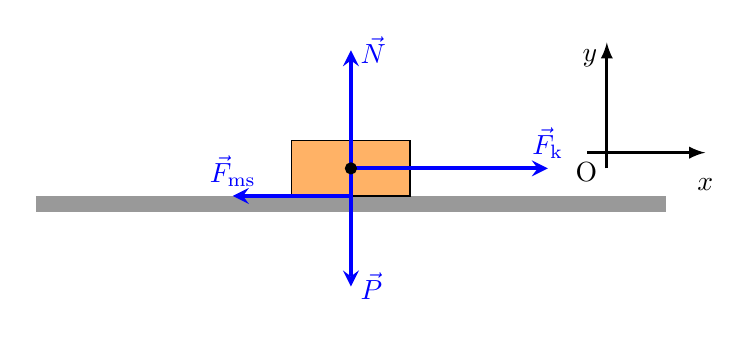
\begin{tikzpicture}
			\coordinate(O) at (0,0);
			\draw[line width=6pt, gray!80!white] (-4,-0.45)--(4,-0.45);
			\filldraw [fill=orange!60!white, draw=black] (-0.75,-0.35) rectangle (0.75,0.35);
			\draw[line width=1.5pt, blue, -stealth] (O)--(2.5,0);
			\draw[line width=1.5pt, blue, -stealth] (0,-0.35)--(-1.5,-0.35);
			\draw[line width=1.5pt, blue, -stealth] (O)--+(0,1.5);
			\draw[line width=1.5pt, blue, -stealth] (O)--+(0,-1.5);
			\filldraw  (O) circle(2pt);
			\node[above, blue] at (2.5,0) {$\vec{F}_{\mathrm{k}}$};
			\node[above, blue] at (-1.5,-0.35) {$\vec{F}_{\mathrm{ms}}$};
			\node[right, blue] at (0,-1.5) {$\vec{P}$};
			\node[right, blue] at (0,1.5) {$\vec{N}$};
			\draw[line width=1pt, -latex] (3,0.2)--(4.5,0.2);
			\draw[line width=1pt, -latex] (3.25,0)--(3.25,1.6);
			\node[below left]at(3.25,0.2) {O};
			\node[below] at(4.5,0) {$x$};
			\node[left] at(3.25,1.4) {$y$};
		\end{tikzpicture}
	\end{center}
	Áp dụng định luật II Newton:
	\begin{equation}
		\label{eq: 3}
		\vec{P}+\vec{N}+\vec{F}_{\mathrm{k}}+\vec{F}_{\mathrm{ms}}=m\vec{a}
	\end{equation}
	Chiếu phương trình \eqref{eq: 3} lên trục $Oy$, ta thu được:
	$$-P+N=0\Rightarrow N=P=mg.$$
	Chiếu phương trình \eqref{eq: 3} lên trục $Ox$, ta thu được:
	$$F_{\mathrm{k}}-F_{\mathrm{ms}}=ma \Leftrightarrow F_{\mathrm{k}}-\mu N=ma.$$
\end{dang}
\begin{vd}
\immini{Một quả khúc côn cầu chuyển động với tốc độ $\SI{20.0}{\meter/\second}$ sau một cú đánh. Quả khúc côn cầu này vẫn có thể trượt chậm dần đều một đoạn $\SI{1.20E2}{\meter}$ trên mặt sân trước khi dừng lại. Xác định hệ số ma sát trượt của nó với mặt sân.}{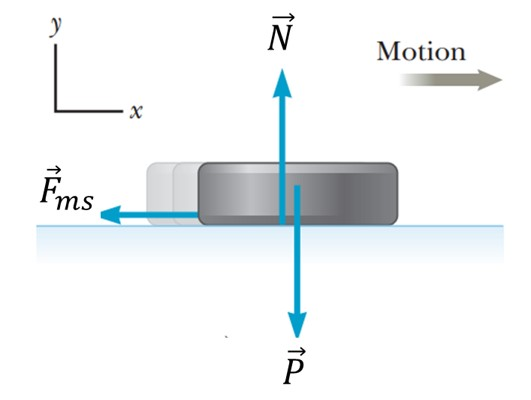
\includegraphics[scale=0.4]{figs/BTMASAT-1}}
\null\hfill\textit{ĐS: $0,17$.}
	\loigiai{}
\end{vd}
\begin{vd}
	Một tủ lạnh có khối lượng $\SI{120}{\kilogram}$ được kéo trượt trên mặt sàn nằm ngang. Biết hệ số ma sát trượt giữa tủ lạnh và mặt sàn là $\mu=0,3$. Lấy gia tốc rơi tự do $g=\SI{9.8}{\meter/\second^2}$.
	\begin{enumerate}[label=\alph*)]
		\item Biết lực kéo có phương nằm ngang và có độ lớn $\SI{500}{\newton}$. Tính gia tốc của tủ lạnh.
		\item Sau thời gian $\SI{10}{\second}$ kể từ lúc kéo, người ta buông tay. Tủ lạnh sẽ chuyển động với gia tốc bằng bao nhiêu? Tính tổng quãng đường tủ lạnh đi được.		
	\end{enumerate}
	\null\hfill\textit{ĐS: a) $a=\SI{1.23}{\meter/\second^2}$, b) $a'=\SI{2.94}{\meter/\second^2}$;  $s'=\SI{86.92}{\meter}$.}
\end{vd}
\begin{dang}{Bài toán lực tác dụng theo phương xiên góc}
	Xét một vật nhỏ khối lượng $m$ chuyển động trên mặt phẳng ngang dưới tác dụng của lực kéo $\vec{F}_{\mathrm{k}}$ theo xiên góc $\alpha$ so với phương ngang. Hệ số ma sát trượt giữa vật và mặt phẳng ngang là $\mu$.
\begin{center}
	\begin{longtable}{M{8cm}M{9cm}}
		\begin{tikzpicture}
			\coordinate(O) at (0,0);
			\coordinate(F) at ($(O)+(30:2.5)$);
			\coordinate(A) at ($(O)+(2.5,0)$);
			
			\draw[line width=6pt, gray!80!white] (-4,-0.45)--(4,-0.45);
			\filldraw [fill=orange!60!white, draw=black] (-0.75,-0.35) rectangle (0.75,0.35);
			\tkzMarkAngle[size=1cm,color=red, line width=1pt](A,O,F);
			\tkzLabelAngle[color=black,pos=1.3, red](A,O,F){$\alpha$};
			\draw[line width=1.5pt, blue, -stealth] (O)--(F);
			\draw[line width=1.5pt, blue, -stealth] (0,-0.35)--(-1.5,-0.35);
			\draw[line width=1.5pt, blue, -stealth] (O)--+(0,1.5);
			\draw[line width=1.5pt, blue, -stealth] (O)--+(0,-1.5);
			\draw[line width=1pt, dashed] (O)--(A);
			\filldraw  (O) circle(2pt);
			\node[above, blue] at (F) {$\vec{F}_{\mathrm{k}}$};
			\node[above, blue] at (-1.5,-0.35) {$\vec{F}_{\mathrm{ms}}$};
			\node[right, blue] at (0,-1.5) {$\vec{P}$};
			\node[right, blue] at (0,1.5) {$\vec{N}$};
		\end{tikzpicture}
		&
		\begin{tikzpicture}
			\coordinate(O) at (0,0);
			\coordinate(F) at ($(O)+(-30:2.5)$);
			\coordinate(A) at ($(O)+(2.2,0)$);
			
			\draw[line width=6pt, gray!80!white] (-4,-0.45)--(4,-0.45);
			\filldraw [fill=orange!60!white, draw=black] (-0.75,-0.35) rectangle (0.75,0.35);
			\tkzMarkAngle[size=1cm,color=red, line width=1pt](F,O,A);
			\tkzLabelAngle[color=black,pos=1.3, red](F,O,A){$\alpha$};
			\draw[line width=1.5pt, blue, -stealth] (O)--(F);
			\draw[line width=1.5pt, blue, -stealth] (0,-0.35)--(-1.5,-0.35);
			\draw[line width=1.5pt, blue, -stealth] (O)--+(0,1.5);
			\draw[line width=1.5pt, blue, -stealth] (O)--+(0,-1.5);
			\draw[line width=1pt, dashed] (O)--(A);
			\filldraw  (O) circle(2pt);
			\node[above, blue] at (F) {$\vec{F}_{\mathrm{k}}$};
			\node[above, blue] at (-1.5,-0.35) {$\vec{F}_{\mathrm{ms}}$};
			\node[right, blue] at (0,-1.5) {$\vec{P}$};
			\node[right, blue] at (0,1.5) {$\vec{N}$};
			\draw[line width=1pt, -latex] (3,0.2)--(4.5,0.2);
			\draw[line width=1pt, -latex] (3.25,0)--(3.25,1.6);
			\node[below left]at(3.25,0.2) {O};
			\node[below] at(4.5,0) {$x$};
			\node[left] at(3.25,1.4) {$y$};
		\end{tikzpicture}
		\\
		\textit{Lực kéo $\vec{F}_{\mathrm{k}}$ chếch lên} &	\textit{Lực kéo $\vec{F}_{\mathrm{k}}$ chếch xuống}
	\end{longtable}
\end{center}
		Áp dụng định luật II Newton:
		\begin{equation}
			\label{eq: 4}
			\vec{P}+\vec{N}+\vec{F}_{\mathrm{k}}+\vec{F}_{\mathrm{ms}}=m\vec{a}
		\end{equation}
		Chiếu phương trình \eqref{eq: 4} lên trục $Oy$, ta thu được:
		\begin{center}
			\begin{tabular}{M{9cm}|M{9cm}}
				\thead{Trường hợp $\vec{F}_{\mathrm{k}}$ chếch lên} & \thead{Trường hợp $\vec{F}_{\mathrm{k}}$ chếch xuống}\\
				$-P+N+F\sin\alpha=0$ & $-P+N-F\sin\alpha=0$\\
				$\Rightarrow N=P-F\sin\alpha$ &$\Rightarrow N=P+F\sin\alpha$
			\end{tabular}
		\end{center}
		Chiếu phương trình \eqref{eq: 4} lên trục $Ox$, ta thu được:
		$$F\cos\alpha-F_{\mathrm{ms}}=ma\Leftrightarrow F\cos\alpha-\mu N=ma.$$
\end{dang}
\begin{vd}
	Phúc và Hạnh có chuyến đi chơi tại khu trượt tuyết. Hạnh ngồi trên chiếc xe trượt tuyết và nhờ Phúc làm cho chiếc xe di chuyển. Phúc có 2 lựa chọn:
	\begin{center}
		\begin{tabular}{M{8cm}M{8cm}}
			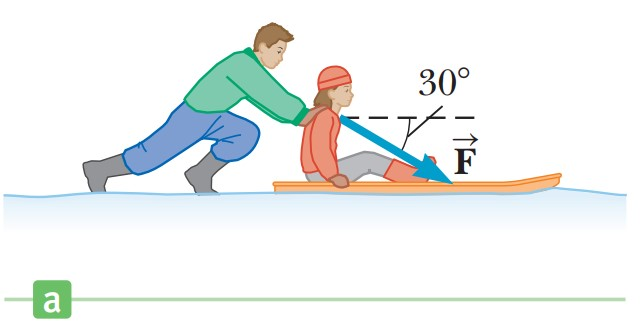
\includegraphics[scale=0.6]{figs/BTMASAT-2}& 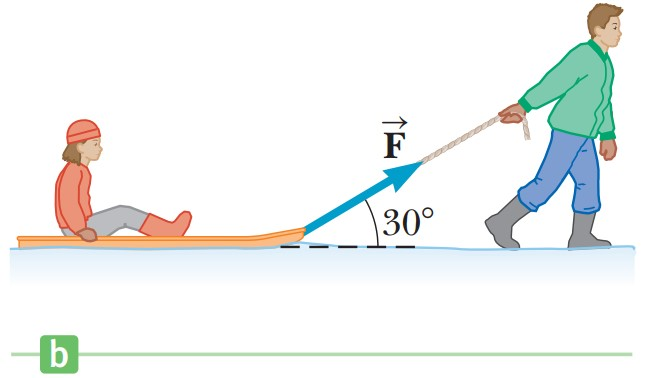
\includegraphics[scale=0.6]{figs/BTMASAT-3}
		\end{tabular}
	\end{center}
	\begin{enumerate}[label=\bfseries Lựa chọn \arabic*:, leftmargin=2.75cm]
		\item Đẩy Hạnh từ phía sau bằng cách tác dụng lực lên vai cô ấy theo hướng xuống dưới và làm với phương ngang góc $\SI{30}{\degree}$ (Hình a).
		\item Kéo xe bằng sợi dây và lực kéo làm với phương ngang góc $\SI{30}{\degree}$ (Hình b).\\
	\end{enumerate}
Cách nào Phúc sẽ cần tác dụng lực ít hơn? Hãy giải thích tại sao.\\
\null\hfill\textit{ĐS: Hai người chia tay rồi \LARGE\Laughey}
\loigiai{}
\end{vd}
\begin{vd}
	\immini{Một người phụ nữ ở sân bay đang kéo một chiếc va li nặng $\SI{20.0}{\kilogram}$ nhờ một sợi dây nhẹ, sợi dây làm với phương ngang góc $\theta$. Va li chuyển động thẳng đều trên mặt sàn. Biết lực kéo của người này là $\SI{35.0}{\newton}$, lực ma sát giữa va li và mặt sàn là $\SI{20.0}{\newton}$.
	\begin{enumerate}[label=\alph*)]
		\item Xác định góc $\theta$.
		\item Tính độ lớn phản lực của mặt sàn tác dụng lên va li.
		\item Xác định hệ số ma sát giữa va li và mặt sàn.
	\end{enumerate}
	}
	{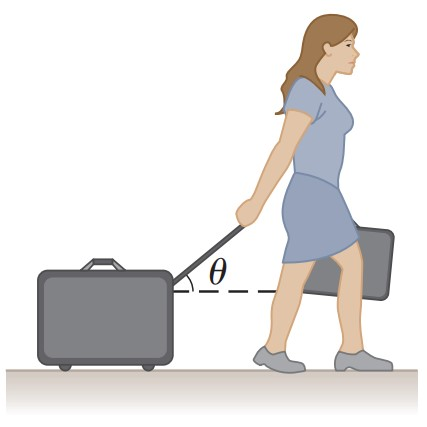
\includegraphics[scale=0.5]{figs/BTMASAT-4}}
	\null\hfill\textit{ĐS: a) $\SI{55.2}{\degree}$, b) $\SI{171.3}{\newton}$, c) $0,12$.}
\end{vd}
\begin{dang}{Bài toán chuyển động của vật trên mặt phẳng nghiêng}
	\begin{center}
		\begin{tabular}{M{8cm}M{8cm}}
			\begin{tikzpicture}
				\coordinate (A) at(0,0);
				\coordinate (B) at($(A)+(150:8)$);
				\coordinate (C) at(-6.928,0);
				\coordinate (O) at(-4,2.8);
				\coordinate (O1) at(-4.2,2.425);
				\coordinate (P) at($(O)+(0,-2.5)$);
				\coordinate (N) at($(O)+(60:2.17)$);
				\coordinate (N') at($(N)+(240:5)$);
				\coordinate (Fms) at($(O1)+(150:1)$);
				\coordinate (O') at(-1,1);
				\coordinate (x) at($(O')+(-30:1)$);
				\coordinate (y) at($(O')+(60:1)$);
				\coordinate (Px) at($(O)+(-30:1.25)$);
				\coordinate (Py) at($(O)+(-120:2.165)$);
				\tkzMarkAngle[size=1cm,color=red, line width=1pt](B,A,C);
				\tkzLabelAngle[color=black,pos=1.3, red](B,A,C){$\alpha$};
				\tkzMarkAngle[size=1cm,color=red, line width=1pt](N',O,P);
				\tkzLabelAngle[color=black,pos=1.3, red](N',O,P){$\alpha$};
				\draw[line width=1pt] (A)--(B)--(C)--(A);
				\node [draw, thick, shape=rectangle, minimum width=1.2cm, minimum height=0.8cm,fill=orange!80!white, rotate=-30] at (O) {};
				\draw[line width=1pt, dashed] (N)--(N');
				\draw[line width=1pt, dashed] (O)--($(O)+(-30:2)$);
				\draw[line width=1pt, gray, dashed] (Py)--(P)--(Px);
				\draw[line width=1.5pt, blue, -stealth] (O)--(P);
				\draw[line width=1.5pt, blue, -stealth] (O)--(N);
				\draw[line width=1.5pt, blue, -stealth] (O1)--(Fms);
				\draw[line width=1.5pt, teal, -stealth] (O)--(Px);
				\draw[line width=1.5pt, teal, -stealth] (O)--(Py);
				\draw[line width=1pt,-latex] (O')--(x);
				\draw[line width=1pt,-latex] (O')--(y);
				\node[right, blue] at(N) {$\vec{N}$};
				\node[right, blue] at(P) {$\vec{P}$};
				\node[above, blue] at(Fms) {$\vec{F}_{\mathrm{ms}}$};
				\node[left] at (O') {O};
				\node[above right] at (x) {$x$};
				\node[above left] at (y) {$y$};
				\node[above, teal] at (Px) {$\vec{P}_x$};
				\node[left, teal] at (Py) {$\vec{P}_y$};
			\end{tikzpicture}&
			\begin{tikzpicture}
				\coordinate (A) at(0,0);
				\coordinate (B) at($(A)+(150:8)$);
				\coordinate (C) at(-6.928,0);
				\coordinate (O) at(-4,2.8);
				\coordinate (O1) at(-4.2,2.425);
				\coordinate (P) at($(O)+(0,-2.5)$);
				\coordinate (N) at($(O)+(60:2.17)$);
				\coordinate (N') at($(N)+(240:5)$);
				\coordinate (Fms) at($(O1)+(-30:2)$);
				\coordinate (O') at(-1,1);
				\coordinate (x) at($(O')+(150:1)$);
				\coordinate (y) at($(O')+(60:1)$);
				\coordinate (Px) at($(O)+(-30:1.25)$);
				\coordinate (Py) at($(O)+(-120:2.165)$);
				\coordinate (v0) at($(O)+(150:2)$);
				\tkzMarkAngle[size=1cm,color=red, line width=1pt](B,A,C);
				\tkzLabelAngle[color=black,pos=1.3, red](B,A,C){$\alpha$};
				\tkzMarkAngle[size=1cm,color=red, line width=1pt](N',O,P);
				\tkzLabelAngle[color=black,pos=1.3, red](N',O,P){$\alpha$};
				\draw[line width=1pt] (A)--(B)--(C)--(A);
				\node [draw, thick, shape=rectangle, minimum width=1.2cm, minimum height=0.8cm,fill=orange!80!white, rotate=-30] at (O) {};
				\draw[line width=1pt, dashed] (N)--(N');
				\draw[line width=1pt, dashed] (O)--($(O)+(-30:2)$);
				\draw[line width=1pt, gray, dashed] (Py)--(P)--(Px);
				\draw[line width=1.5pt, blue, -stealth] (O)--(P);
				\draw[line width=1.5pt, blue, -stealth] (O)--(N);
				\draw[line width=1.5pt, blue, -stealth] (O1)--(Fms);
				\draw[line width=1.5pt, teal, -stealth] (O)--(Px);
				\draw[line width=1.5pt, teal, -stealth] (O)--(Py);
				\draw[line width=1pt,-latex] (O')--(x);
				\draw[line width=1pt,-latex] (O')--(y);
				\node[right, blue] at(N) {$\vec{N}$};
				\node[right, blue] at(P) {$\vec{P}$};
				\node[below, blue] at(Fms) {$\vec{F}_{\mathrm{ms}}$};
				\node[right] at (O') {O};
				\node[above right] at (x) {$x$};
				\node[right] at (y) {$y$};
				\node[above, teal] at (Px) {$\vec{P}_x$};
				\node[left, teal] at (Py) {$\vec{P}_y$};
				\draw[red, -latex, line width=1.5pt] (O)--(v0);
				\node[above, red] at (v0) {$\vec{v}_0$};
			\end{tikzpicture}\\
			\textit{Vật trượt xuống} & \textit{Vật trượt lên}
		\end{tabular}	
	\end{center}
	Áp dụng định luật II Newton:
	\begin{equation}
		\label{eq: 5}
		\vec{P}+\vec{N}+\vec{F}_{\mathrm{ms}}=m\vec{a}
	\end{equation}
	Chiếu phương trình \eqref{eq: 5} lên phương $Oy$:
	$$-Py+N=0\Rightarrow N=P_y=mg\cos\alpha.$$
	Chiếu phương trình \eqref{eq: 5} lên phương $Ox$:
	\begin{center}
		\begin{tabular}{M{8cm}|M{8cm}}
			\thead{Trường hợp vật trượt xuống}& \thead{Trường hợp vật trượt lên}\\
			$P_x-F_{\mathrm{ms}}=ma$ & $-P_x-F_{\mathrm{ms}}=ma$\\
			$\Leftrightarrow mg\sin\alpha-\mu N=ma$ & 
			$\Leftrightarrow -mg\sin\alpha-\mu N=ma$
		\end{tabular}
	\end{center}
\end{dang}
\begin{vd}
	Một vật trượt đều trên mặt phẳng nghiêng có chiều dài $\SI{2}{\meter}$, chiều cao $h=\SI{0.5}{\meter}$. Hãy tính hệ số ma sát trượt giữa vật và mặt phẳng nghiêng.\\
	\null\hfill\textit{ĐS: $\mu\approx0,26$.}
\end{vd}
\begin{vd}
	\immini{Một vật nhỏ khối lượng $m=\SI{5.8}{\kilogram}$ được kéo trượt trên mặt phẳng nghiêng góc $\theta=\SI{25}{\degree}$ so với phương ngang như hình vẽ. Độ lớn lực kéo tác dụng lên vật là $F=\SI{32}{\newton}$. Lấy gia tốc trọng trường $g=\SI{9.8}{\meter/\second^2}$.
	\begin{enumerate}[label=\alph*)]
		\item Xác định độ lớn gia tốc của vật trong trường hợp mặt nghiêng hoàn toàn nhẵn.
		\item Xác định độ lớn gia tốc của vật nếu hệ số ma sát trượt giữa vật và mặt nghiêng là $0,10$.
	\end{enumerate}
	}
	{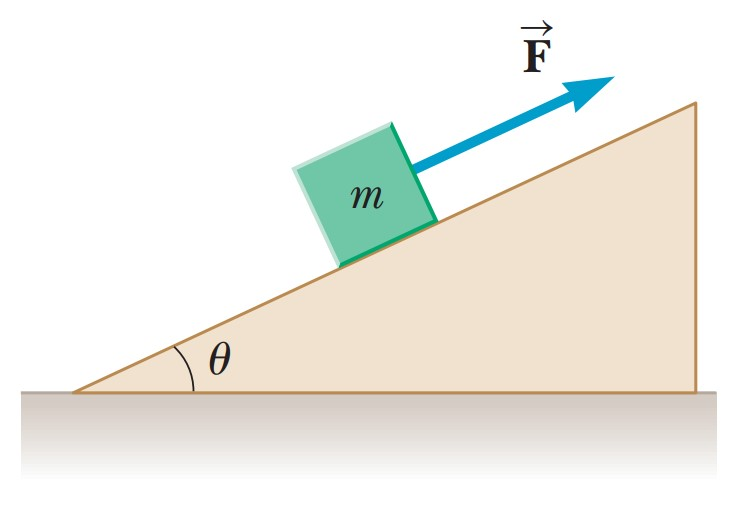
\includegraphics[scale=0.4]{figs/BTMASAT-5}}
	\null\hfill\textit{ĐS: a) $a\approx\SI{1.38}{\meter/\second^2}$, b) $a'\approx\SI{0.49}{\meter/\second^2}$.}
\end{vd}
\subsubsection{Điều kiện cân bằng lực}
Vật ở trạng thái cân bằng lực (vật đứng yên hoặc chuyển động thẳng đều) khi hợp lực tác dụng lên nó bằng không:
\begin{equation}
	\label{eq: 6}
	\sum\vec{F}=\vec{0}
\end{equation}
\begin{dang}{Bài toán cân bằng của vật treo bằng dây nhẹ, không dãn}
	Vật ở trạng thái cân bằng lực khi tổng hợp lực tác dụng lên vật bằng không:
	\begin{equation}
		\label{eq: 7}
		\sum\vec{F}=\vec{F}_1+\vec{F}_2+\dots+\vec{F}_n=\vec{0}
	\end{equation}
	Để giải phương trình \eqref{eq: 7}, thông thường ta có thể sử dụng 2 cách:
	\begin{itemize}
		\item \textbf{Cách 1:} Chọn hệ trục tọa độ vuông góc $Oxy$ rồi chiếu phương trình \eqref{eq: 7} lên các trục $Ox$ và $Oy$ tương ứng.
		\item \textbf{Cách 2:} Sử dụng quy tắc đa giác vector. Hợp lực của các lực tác dụng lên vật bằng không nên các lực tác dụng lên vật sẽ tạo thành đa giác vector khép kín.
	\end{itemize}
\end{dang}
\begin{vd}
	\immini{Một tên trộm đang trèo tường để đào thoát bằng một sợi dây như hình minh họa. Trọng lượng của tên trộm này là $\SI{600}{\newton}$. 
		\begin{enumerate}[label=\alph*)]
			\item Xác định lực căng trên mỗi dây.
			\item Nếu điểm treo của sợi dây nằm ngang được đặt ở vị trí cao hơn trên tường thì lực căng của sợi dây bên kia sẽ thay đổi như thế nào?
		\end{enumerate}
		}
	{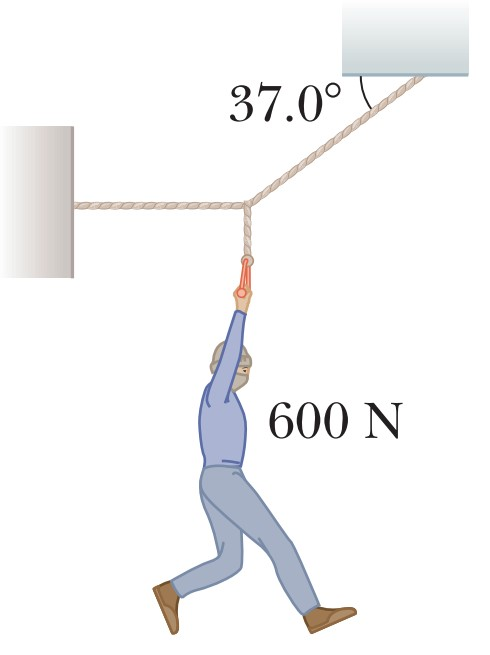
\includegraphics[scale=0.4]{figs/BTMASAT-6}}
	\null\hfill \textit{ĐS: a) Lực căng trên dây xiên góc $\SI{997}{\newton}$ và lực căng trên dây nằm ngang $\SI{796}{\newton}$, b) \LARGE\Laughey.}
\end{vd}
\begin{dang}{Bài toán cân bằng của vật trong chất lỏng}
Khi vật chìm trong chất lỏng, vật chịu thêm tác dụng của lực đẩy Archimedes.\\
\textbf{Lực đẩy Archimedes} tác dụng lên vật có điểm đặt tại vị trí trùng với trọng tâm của phần chất lỏng bị vật chiếm chỗ, có phương thẳng đứng, có chiều từ dưới lên trên, có độ lớn bằng trọng lượng phần chất lỏng bị chiếm vật chiếm chỗ.
$$F=\rho gV$$
Trong đó:
\begin{itemize}
	\item $\rho$: khối lượng riêng của chất lỏng $\left(\si{\kilogram/\meter^3}\right)$;
	\item $g$: gia tốc trọng trường $\left(\si{\meter/\second^2}\right)$;
	\item $V$: thể tích phần chất lỏng bị vật chiếm chỗ $\left(\si{\meter^3}\right)$.
\end{itemize}
\end{dang}
\begin{vd}
	\immini{Vào năm 231, một chiếc vương miện mới đã được chế tạo cho Vua Hiero II. Nhà vua yêu cầu Archimedes xác định liệu vương miện có phải được sử dụng vàng ròng hay được pha thêm bạc bởi một người thợ bất lương. Archimedes phải giải quyết vấn đề mà không được làm hư hại chiếc vương miện, do đó ông tiến thành thí nghiệm như hình minh họa bên. }
	{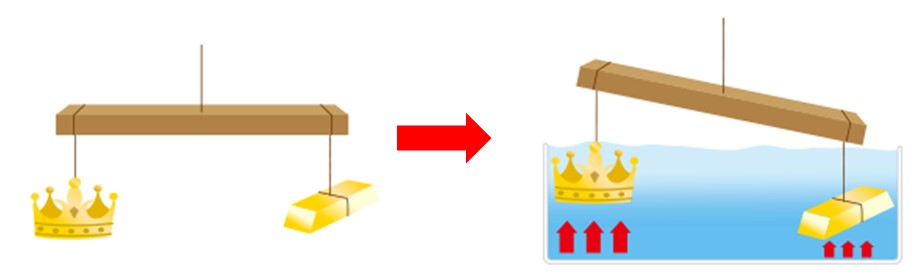
\includegraphics[scale=0.6]{figs/BTMASAT-8}}
	Dựa vào kiến thức đã học, em hãy giải thích cơ sở khoa học của thí nghiệm do Archimedes thực hiện. Biết rằng bạc có khối lượng riêng nhỏ hơn vàng.\\
	\null\hfill\textit{ĐS: Dễ quá dễ quá \LARGE\Laughey}
\end{vd}
\begin{vd}
	\immini{Một khối gỗ hình hộp chữ nhật có diện tích đáy $S=\SI{40}{\centi\meter^2}$ và cao $h=\SI{10}{\centi\meter}$. Khối lượng của khối gỗ $m=\SI{160}{\gram}$. Khối lượng riêng của nước là $\rho=\SI{1000}{\kilogram/\meter^3}$. Thả khối gỗ vào nước, khối gỗ nổi lơ lửng trên mặt nước như hình vẽ. Tìm chiều cao của phần gỗ nổi trên mặt nước.}
	{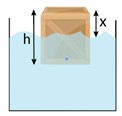
\includegraphics[scale=0.7]{figs/BTMASAT-7}	
	}
	\null\hfill\textit{ĐS: $x=\SI{6}{\centi\meter}$.}
\end{vd}
\end{tomtat}
